\documentclass{article}
\usepackage{geometry} \geometry{margin=1in}
\usepackage{parskip}
\usepackage{ragged2e}
\usepackage{float}
\usepackage{tcolorbox}
\usepackage{amsmath, amssymb}
\usepackage{tikz} \usetikzlibrary{shapes, arrows.meta, positioning, shadows, fit, calc}
\usepackage{hyperref}

% MANDATORY STYLE DEFINITIONS
\tikzset{
    block/.style={rectangle, draw, thick, rounded corners, fill=blue!5, align=center, minimum height=2em},
    process/.style={rectangle, draw, fill=blue!10, align=center},
    decision/.style={diamond, draw, fill=green!10, align=center, aspect=2},
    arrow/.style={thick, ->, >=stealth},
    data/.style={circle, draw, thick, fill=orange!10, minimum size=1.5em}
}
\raggedbottom

\begin{document}

\title{Cybersecurity (CSCI 2413): Final Review}
\author{Student Companion Guide}
\date{\today}
\maketitle

\section{Introduction to Cybersecurity Review}

This companion guide summarizes the critical concepts reviewed for Cybersecurity, CSCI 2413, focusing on foundational knowledge, penetration testing methodologies, common web application vulnerabilities as defined by the OWASP Top Ten (2021), and defensive strategies.

\section{Protocols and Ports}

A fundamental requirement in networking and security is understanding which common protocols operate on which ports. This knowledge is essential for firewall configuration, intrusion detection, and performing reconnaissance during penetration testing.

\begin{tcolorbox}[title=Common Protocols and Ports]
\begin{center}
\begin{tabular}{|l|l|}
\hline
\textbf{Protocol} & \textbf{Port} \\
\hline
FTP (File Transfer Protocol) & 20, 21 \\
\hline
SSH (Secure Shell) & 22 \\
\hline
Telnet (Telecommunication Network) & 23 \\
\hline
SMTP (Simple Mail Transfer Protocol) & 25 \\
\hline
DNS (Domain Name System) & 53 \\
\hline
HTTP (Hypertext Transfer Protocol) & 80 \\
\hline
POP3 (Post Office Protocol version 3) & 110 \\
\hline
LDAP (Lightweight Directory Access Protocol) & 389 \\
\hline
HTTPS (HTTP Secure) & 443 \\
\hline
RDP (Remote Desktop Protocol) & 3389 \\
\hline
\end{tabular}
\end{center}
\end{tcolorbox}
It is crucial to note that services running on low-numbered ports (1-1023) are often privileged and require administrative rights to bind to. Modern secure equivalents, like HTTPS (443) for HTTP (80), or SSH (22) for Telnet (23) and FTP (21, 20), should always be preferred to prevent eavesdropping and data tampering.

\section{Types of Hackers and Penetration Testing}

The cybersecurity industry categorizes individuals who attempt to bypass security measures into different ``hats,'' reflecting their intent and legality.

\subsection{Types of Hackers}

\begin{itemize}
    \item \textbf{White Hat Hacker (Ethical Hacker):} This individual is usually referred to as a penetration tester today. They operate with explicit permission from the asset owners to simulate attacks against a target system. Their goal is defensive: to find vulnerabilities before malicious actors do.
    \item \textbf{Black Hat Hacker (Cracker):} These are malicious actors who gain unauthorized access to systems with the intent to cause harm, disruption, or financial gain. They act illegally and without permission.
    \item \textbf{Gray Hat Hacker:} A complex category, the gray hat hacker typically acts as a law-abiding citizen but may sometimes venture into unauthorized activities, often believing their actions are justified, such as exposing vulnerabilities publicly without prior consent from the owner.
\end{itemize}

\subsection{Penetration Testing (PenTester)}

A Penetration Tester (PenTester) is an ethical hacker who is formally \textbf{AUTHORIZED} to simulate a cyberattack against a computer or server environment. Pen Testers are typically employed by specialized security firms that perform structured attacks on behalf of a client. Their deliverables include a comprehensive report detailing any vulnerabilities found and concrete recommendations on how to remediate those issues.

\subsubsection{Penetration Testing Stages (Conceptual Model)}

The penetration testing process is usually broken down into several distinct phases to ensure thoroughness and repeatability. Intuitively, this involves preparation, discovery, exploitation, sustained access, and final reporting/configuration validation.

\begin{figure}[H]
\centering
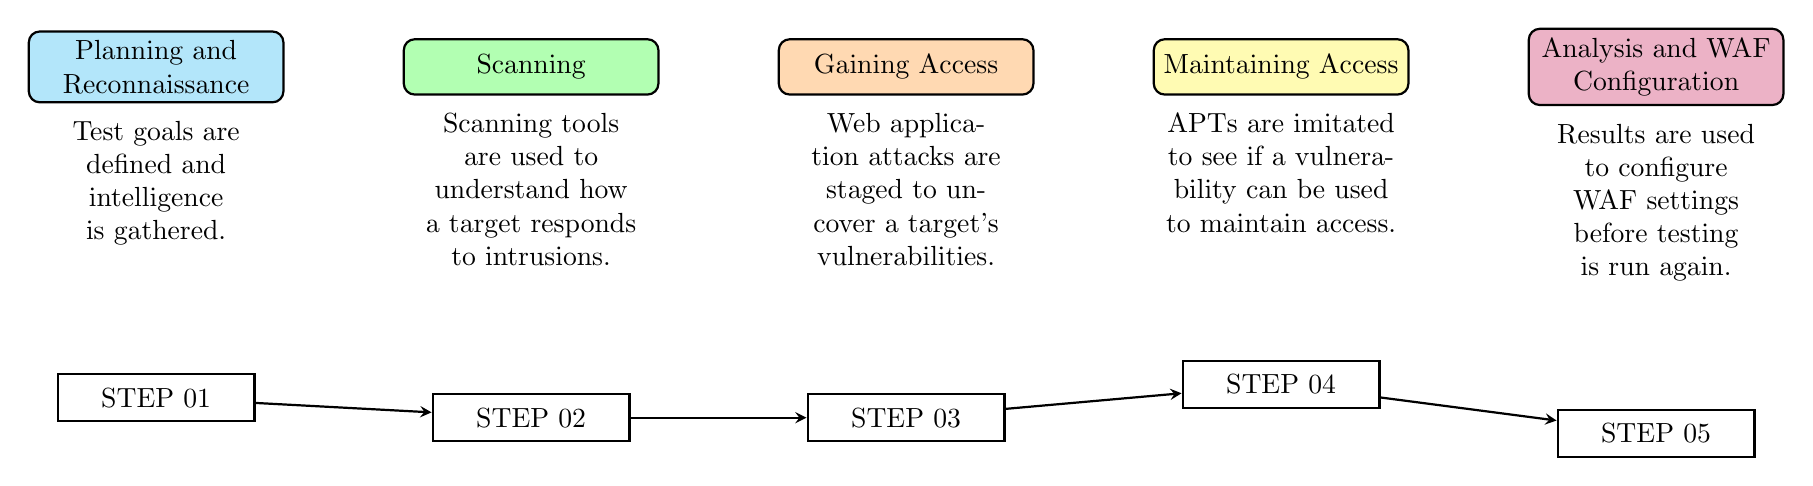
\begin{tikzpicture}[node distance=2cm]

    % Nodes
    \node (p1) [block, fill=cyan!30, text width=3cm] {Planning and \\ Reconnaissance};
    \node (p2) [block, right=1.5cm of p1, fill=green!30, text width=3cm] {Scanning};
    \node (p3) [block, right=1.5cm of p2, fill=orange!30, text width=3cm] {Gaining Access};
    \node (p4) [block, right=1.5cm of p3, fill=yellow!30, text width=3cm] {Maintaining Access};
    \node (p5) [block, right=1.5cm of p4, fill=purple!30, text width=3cm] {Analysis and WAF \\ Configuration};

    % Descriptions
    \node [below=0.1cm of p1, text width=3cm, align=center] (d1) {Test goals are defined and intelligence is gathered.};
    \node [below=0.1cm of p2, text width=3cm, align=center] (d2) {Scanning tools are used to understand how a target responds to intrusions.};
    \node [below=0.1cm of p3, text width=3cm, align=center] (d3) {Web application attacks are staged to uncover a target's vulnerabilities.};
    \node [below=0.1cm of p4, text width=3cm, align=center] (d4) {APTs are imitated to see if a vulnerability can be used to maintain access.};
    \node [below=0.1cm of p5, text width=3cm, align=center] (d5) {Results are used to configure WAF settings before testing is run again.};
    
    % Steps
    \node [below=1.5cm of d1, draw, thick, inner sep=5pt, fill=white, minimum width=2.5cm] (s1) {STEP 01};
    \node [below=1.5cm of d2, draw, thick, inner sep=5pt, fill=white, minimum width=2.5cm] (s2) {STEP 02};
    \node [below=1.5cm of d3, draw, thick, inner sep=5pt, fill=white, minimum width=2.5cm] (s3) {STEP 03};
    \node [below=1.5cm of d4, draw, thick, inner sep=5pt, fill=white, minimum width=2.5cm] (s4) {STEP 04};
    \node [below=1.5cm of d5, draw, thick, inner sep=5pt, fill=white, minimum width=2.5cm] (s5) {STEP 05};

    % Arrows
    \draw [arrow] (s1) -- (s2);
    \draw [arrow] (s2) -- (s3);
    \draw [arrow] (s3) -- (s4);
    \draw [arrow] (s4) -- (s5);

\end{tikzpicture}
\caption{Conceptual Penetration Testing Workflow}
\end{figure}

\subsubsection{Penetration Testing Stages (Technical Model)}

A more detailed, technical perspective on the stages of a penetration test reveals an iterative process focusing heavily on discovery and escalation.

\begin{figure}[H]
\centering
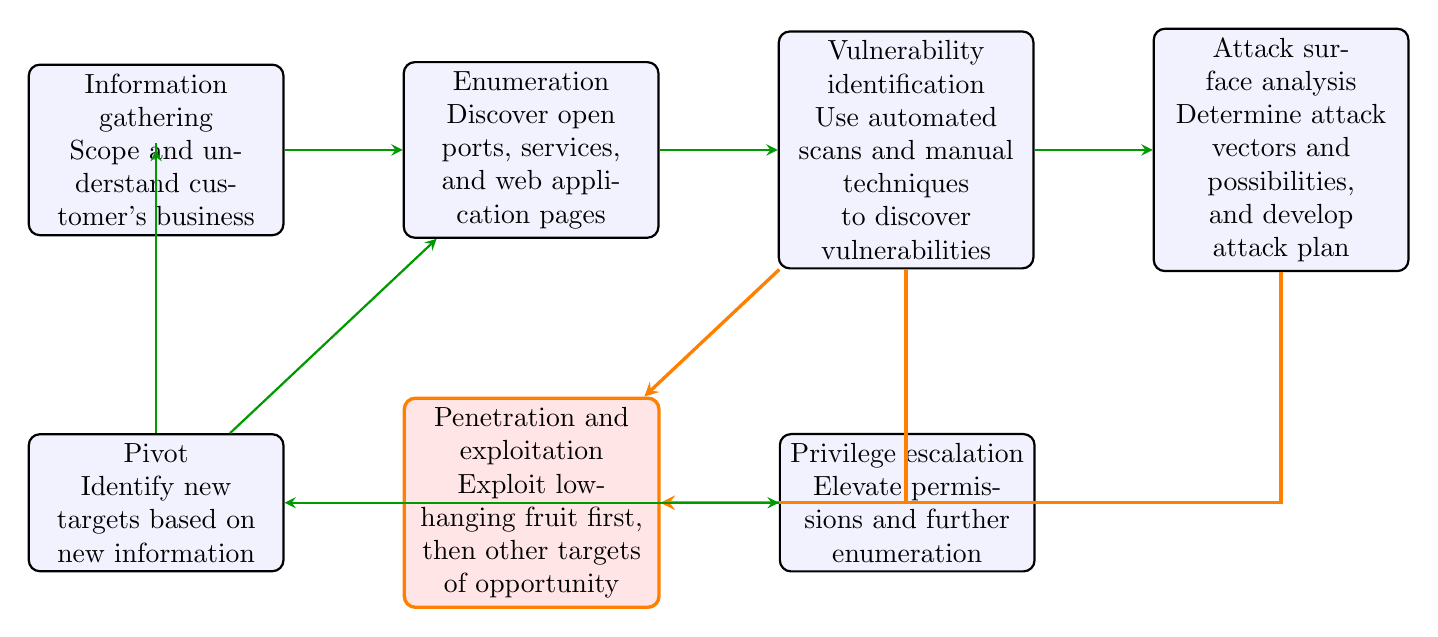
\begin{tikzpicture}[node distance=2.5cm, >=stealth]

    % Top Row Nodes
    \node (info) [block, text width=3cm] {Information gathering \\ Scope and understand customer's business};
    \node (enum) [block, right=1.5cm of info, text width=3cm] {Enumeration \\ Discover open ports, services, and web application pages};
    \node (vuln) [block, right=1.5cm of enum, text width=3cm] {Vulnerability identification \\ Use automated scans and manual techniques to discover vulnerabilities};
    \node (attack) [block, right=1.5cm of vuln, text width=3cm] {Attack surface analysis \\ Determine attack vectors and possibilities, and develop attack plan};

    % Bottom Row Nodes
    \node (pivot) [block, below=2.5cm of info, text width=3cm] {Pivot \\ Identify new targets based on new information};
    \node (exploit) [block, right=1.5cm of pivot, text width=3cm, draw=orange, very thick, fill=red!10] {Penetration and exploitation \\ Exploit low-hanging fruit first, then other targets of opportunity};
    \node (priv) [block, right=1.5cm of exploit, text width=3cm] {Privilege escalation \\ Elevate permissions and further enumeration};
    
    % Arrows (Forward flow)
    \draw [arrow, color=green!60!black] (info) -- (enum);
    \draw [arrow, color=green!60!black] (enum) -- (vuln);
    \draw [arrow, color=green!60!black] (vuln) -- (attack);
    
    % Main Attack/Exploitation flow
    \draw [arrow, color=orange, very thick] (attack) |- (exploit);
    \draw [arrow, color=orange, very thick] (vuln) -- (exploit);
    \draw [arrow, color=orange, very thick] (vuln) |- (exploit);

    % Post-exploitation and looping flow
    \draw [arrow, color=green!60!black] (exploit) -- (priv);
    \draw [arrow, color=green!60!black] (priv) -- (pivot);
    \draw [arrow, color=green!60!black] (pivot) |- (info); % Loop back to info gathering/enumeration if needed
    \draw [arrow, color=green!60!black] (pivot) -- (enum);

\end{tikzpicture}
\caption{Technical Penetration Testing Stages}
\end{figure}

\section{The Open Web Application Security Project (OWASP)}

OWASP is a crucial non-profit foundation dedicated to improving the security of software. They achieve this by providing:
\begin{enumerate}
    \item Tools and resources for testing and development.
    \item A global community platform for networking and collaboration.
    \item Education and training materials on secure coding practices.
\end{enumerate}
The OWASP Top Ten is perhaps their most famous publication, outlining the ten most critical web application security risks. This list is released periodically (typically every 3--4 years), with the current version being from 2021.

When determining the criticality and ranking of vulnerabilities, OWASP assesses several criteria: \textbf{Exploitability}, \textbf{Prevalence}, \textbf{Detectability}, and \textbf{Technical impact}.

\begin{tcolorbox}[title=OWASP Top Ten Comparison (2017 vs. 2021)]
The 2021 list saw significant reshuffling and the introduction of new categories, reflecting changes in development practices (e.g., component usage, design focus) and attack trends (e.g., SSRF).

\begin{tabular}{|p{0.45\textwidth}|p{0.45\textwidth}|}
\hline
\textbf{2017 Rank and Vulnerability} & \textbf{2021 Rank and Vulnerability} \\
\hline
A01:2017-Injection & A01:2021-Broken Access Control (Moved from A05) \\
A02:2017-Broken Authentication & A02:2021-Cryptographic Failures (Previously A03: Sensitive Data Exposure) \\
A03:2017-Sensitive Data Exposure & A03:2021-Injection (Moved from A01) \\
A04:2017-XML External Entities (XXE) & \textbf{A04:2021-Insecure Design (New)} \\
A05:2017-Broken Access Control & A05:2021-Security Misconfiguration (Moved from A06) \\
A06:2017-Security Misconfiguration & A06:2021-Vulnerable and Outdated Components (Moved from A09) \\
A07:2017-Cross-Site Scripting (XSS) & A07:2021-Identification and Authentication Failures (Moved from A02) \\
A08:2017-Insecure Deserialization & \textbf{A08:2021-Software and Data Integrity Failures (New)} \\
A09:2017-Using Components with Known Vulnerabilities & A09:2021-Security Logging and Monitoring Failures (Moved from A10) \\
A10:2017-Insufficient Logging \& Monitoring & \textbf{A10:2021-Server-Side Request Forgery (SSRF) (New/Re-entry)} \\
\hline
\end{tabular}
\end{tcolorbox}

\section{A01: Broken Access Control (2021)}

Access control refers to the policies implemented by an application to ensure that users are restricted to acting within their defined and intended permissions. Failures in this area are severe, often leading to unauthorized information disclosure, modification, or outright destruction of data, or allowing a user to perform business functions far outside their security scope.

\subsection{Vulnerabilities Associated with Access Control}

Broken access control can manifest in numerous ways:
\begin{itemize}
    \item \textbf{Violation of Least Privilege:} Failing to adhere to the principle of least privilege, or not enforcing a ``deny by default'' approach.
    \item \textbf{Parameter Tampering (Bypassing Checks):} Modifying parameters in the URL (e.g., changing an item ID or user ID) to bypass intended access control checks. This allows users to view or edit someone else's account data.
    \item \textbf{Missing Access Controls in APIs:} Accessing API endpoints (particularly those using methods like \texttt{POST}, \texttt{PUT}, or \texttt{DELETE}) that lack sufficient authorization checks.
    \item \textbf{Privilege Elevation:} A user acting as a highly privileged user without having properly authenticated or having the requisite permissions.
    \item \textbf{Metadata Manipulation:} Tampering with session information or authentication tokens, such as replaying or modifying a JSON Web Token (JWT), to gain unwarranted access.
    \item \textbf{Force Browsing:} Navigating directly to authenticated or privileged pages as an unauthenticated or standard user by simply guessing the URL structure.
\end{itemize}

\subsection{Web HTTP Methods and Status Codes}

When discussing web applications and access control, we must understand the core ways a client interacts with a server using HTTP methods (verbs) and how the server responds (status codes).

\subsubsection*{HTTP Methods}
These verbs dictate the intended action on a resource:
\begin{itemize}
    \item \textbf{GET:} Retrieves data from the server.
    \item \textbf{PUT:} Sends updated data to the server (used for modifying an existing resource).
    \item \textbf{POST:} Sends new or created data to the server (used for creating a new resource).
    \item \textbf{DELETE:} Removes data from the server.
\end{itemize}

\subsubsection*{HTTP Status Codes}
These codes are returned by the server to indicate the outcome of the request:
\begin{itemize}
    \item \textbf{20X (Success):} Indicates successful processing.
    \begin{itemize}
        \item 200 -- OK (Standard success)
        \item 201 -- Created (Resource creation successful)
        \item 204 -- No Content (Action successful, but no content returned)
    \end{itemize}
    \item \textbf{30X (Redirection):} Indicates the client needs to take further action.
    \begin{itemize}
        \item 301 -- Moved Permanently
        \item 304 -- Not Modified
    \end{itemize}
    \item \textbf{40X (Client Error):} Indicates the client made a bad request or lacks authorization.
    \begin{itemize}
        \item 400 -- Bad Request (Server cannot process due to client error)
        \item \textbf{401 -- Unauthorized} (Client must authenticate)
        \item \textbf{403 -- Forbidden} (Client is authenticated but lacks necessary permissions)
        \item 404 -- Not Found
    \end{itemize}
    \item \textbf{50X (Server Error):} Indicates the server failed to fulfill the request.
    \begin{itemize}
        \item 500 -- Internal Server Error
        \item 503 -- Service Unavailable
    \end{itemize}
\end{itemize}

\subsection{Prevention: Broken Access Control}
To prevent broken access control vulnerabilities, developers should:
\begin{itemize}
    \item \textbf{Deny by Default:} Always assume a user lacks permission unless explicitly granted access.
    \item \textbf{Implement CORS Safely:} Use Cross-Origin Resource Sharing (CORS) only when necessary and configure origins securely to prevent unauthorized domain access.
    \item \textbf{Restrict File Access:} Disable web server directory listing to prevent attackers from browsing sensitive files.
    \item \textbf{Log and Review Failures:} Log all access control failures and review these logs periodically, treating them as potential hack attempts.
    \item \textbf{Validate Permissions Server-Side:} Always ensure the correct user is making the change and that they possess the necessary permissions, regardless of client-side validation.
    \item \textbf{Use Secure Tokens:} Use tokens like JSON Web Tokens (JWT) (\url{https://jwt.io}) for authentication, but ensure the token data is integrity-protected (signed) and that permissions encoded within it are respected.
    \item \textbf{Avoid Guessable Identifiers:} Make IDs harder to guess, preferably using non-numeric Globally Unique Identifiers (GUIDs) (\url{https://guidgenerator.com/}) instead of simple sequential integers.
\end{itemize}

\section{A02: Cryptographic Failures (2021)}
Previously referred to as A03: Sensitive Data Exposure (2017), this category focuses on protecting data in transit and at rest. This protection is vital for various types of sensitive data:
\begin{itemize}
    \item Passwords
    \item Credit Cards (covered under PCI standards)
    \item Health Records (covered under HIPAA/HIPPA equivalent regulations)
    \item Personal Information (PII)
\end{itemize}

\subsection{Assessing Vulnerability and Data Classification}
To assess whether an application is vulnerable, we must ask critical questions about cryptographic implementation:
\begin{itemize}
    \item Is any sensitive data transmitted in clear text (unencrypted)?
    \item Is the cryptography version deprecated or known to be weak (e.g., SHA1, MD5)?
    \item Are default crypto keys in use, and how were they generated? (Default keys are a huge risk; poor entropy generation leads to weak keys.)
    \item Is the certificate chain validated, and has the certificate expired?
    \item Are the same keys being used across multiple, separate servers? (This violates the principle of key segregation.)
\end{itemize}

Before protecting data, organizations must first classify it to determine its required level of security.

\subsubsection*{Classification Criteria}
\begin{itemize}
    \item Is the data a company secret?
    \item Are there specific legal requirements governing the data (e.g., PII, Health Data)?
    \item Is it highly sensitive authentication data (Password, PIN code, Security Question Answer)?
\end{itemize}

\subsubsection*{Classification and Storage Method}
Once sensitivity is determined, the storage and transmission method must align with the risk:
\begin{itemize}
    \item \textbf{Passwords, PIN codes:} MUST be Hashed (one-way function, irreversible).
    \item \textbf{User personal information, User health information, Company Private Info:} Must be Encrypted (reversible, but protected).
    \item \textbf{Company Public info, User Public info:} Can often be stored as Plain Text.
\end{itemize}
It is important to remember that hashing is suitable for comparison and verification (like passwords), while encryption is required if the data must eventually be retrieved in its original form (like health records or credit card numbers).

\subsection{Secure Transmission and Storage}

\subsubsection*{Data Transmission Protocols}
Non-secure protocols must be avoided in favor of their secure counterparts:
\begin{itemize}
    \item \textbf{HTTP (Web)} is not secure. All websites must use \textbf{HTTPS} (Secure Web), which leverages TLS/SSL encryption.
    \item \textbf{FTP (File Transfer)} is not secure. All servers should use \textbf{FTPS} (Secure File Transfer Protocol), often utilizing SSL/TLS for encryption.
    \item \textbf{SMTP (Mail)} is inherently insecure. While there isn't one universal secure mail protocol, modern mail solutions (like Gmail) support encrypting and decrypting mail, often via STARTTLS or specialized add-ons utilizing Public Key Infrastructure (PKI).
\end{itemize}

\subsubsection*{Secure Email (PKI)}
Secure email relies on Public Key Encryption. Both the sender and receiver possess a public key (used to encrypt data for the other party) and a private key (used to decrypt data intended for them). Implementing this successfully requires coordination between the parties to exchange public keys.

\subsubsection*{Credit Card Data (PCI Compliance)}
The Payment Card Industry (PCI) sets strict standards for storing and handling credit cards. Companies are highly discouraged from storing raw credit card data. The recommended security practice for systems requiring recurring payments is to use a secure token (an encrypted, non-sensitive value) provided by a credit card clearing company, ensuring the application itself never holds the sensitive primary account number (PAN).

\subsection{Prevention: Cryptographic Failures}
Preventing cryptographic failure involves establishing policies around classification and usage:
\begin{itemize}
    \item Classify data processed, stored, or transmitted into defined sensitivity levels.
    \item Ensure classification considers all applicable laws and regulations.
    \item Do not store sensitive data if it is avoidable.
    \item Encrypt all sensitive data at rest using strong, industry-standard cryptography.
    \item Use cryptographic standards that are current and up to date.
    \item \textbf{Mandate TLS 1.2 or above} for all data in transit. TLS 1.3 is strongly preferred.
    \item Disable caching of sensitive data in web browsers or on servers.
\end{itemize}

\section{A03: Injection Attacks (2021)}

Injection flaws occur when untrusted data is sent to an interpreter (like a database, command shell, or LDAP server) without proper validation or sanitization. This allows attackers to execute unintended commands or access data without authorization.

While \textbf{SQL Injection} is the most commonly discussed type, injection attacks include:
\begin{itemize}
    \item SQL (Structured Query Language)
    \item NoSQL (Non-Relational Databases)
    \item Command Injection (OS commands)
    \item LDAP (Lightweight Directory Access Protocol)
\end{itemize}

\subsection{Injection Vulnerability Checklist}
An application is vulnerable to injection if:
\begin{itemize}
    \item User-supplied data is \textbf{NOT validated} for structure, content, or type.
    \item Dynamic queries are built using string concatenation rather than being \textbf{parameterized} (precompiled statements).
    \item Hostile data (input containing malicious code) is directly used or concatenated into the final command/query string.
\end{itemize}

\subsection{Relational Databases and SQL Basics}
Relational databases structure data efficiently into Tables, which contain columns (fields) and rows (records), similar to a spreadsheet. These tables are managed using Structured Query Language (SQL).

\begin{tcolorbox}[title=SQL CRUD Keywords]
SQL operations map directly to the foundational Create, Read, Update, Delete (CRUD) actions:
\begin{itemize}
    \item \textbf{CREATE} = \texttt{INSERT INTO}
    \item \textbf{READ} = \texttt{SELECT}
    \item \textbf{UPDATE} = \texttt{UPDATE}
    \item \textbf{DELETE} = \texttt{DELETE}
\end{itemize}
\end{tcolorbox}

\subsubsection*{READ - SELECT}
The basic syntax retrieves columns from a table:
\begin{verbatim}
SELECT [columns] FROM [table]
\end{verbatim}
The columns list can be one or multiple column names separated by commas, or ``\texttt{*}'' to mean all columns.

\subsubsection*{Filtering with WHERE}
The \texttt{WHERE} clause filters the resulting rows based on specific column values:
\begin{verbatim}
SELECT [columns] FROM [table] WHERE [column] = [value]
\end{verbatim}
The \texttt{LIKE} operator can be used for pattern matching, such as selecting all names that start with 'J': \texttt{WHERE Name LIKE 'J\%'}.

\subsubsection*{CREATE - INSERT INTO}
This statement adds new data rows to a table. Note the strict requirement for matching column and value lists.
\begin{verbatim}
INSERT INTO [table] ([columns]) VALUES ([values])
\end{verbatim}

\subsubsection*{UPDATE - UPDATE}
Used to modify existing data. Need to be extremely cautious: without a \texttt{WHERE} clause, \textbf{all} records in the table will be changed.
\begin{verbatim}
UPDATE [table] SET [column]=[value] WHERE [column]=[value]
\end{verbatim}

\subsubsection*{DELETE - DELETE}
Used to remove data. Need to be \textbf{EXTRA} careful: without a \texttt{WHERE} clause, \textbf{all} records in the table will be deleted.
\begin{verbatim}
DELETE FROM [table] WHERE [column]=[value]
\end{verbatim}

\subsection{The Mechanics of SQL Injection}

SQL Injection works by exploiting applications that construct queries using unprotected user input concatenated into a string. The core vulnerability involves manipulating string concatenation to inject operational SQL commands.

Consider a dynamic query where an attacker substitutes the password input with: \texttt{jmaxwell' or '1'='1' --}

This input modifies the structure of the intended query:
\begin{verbatim}
SELECT * FROM Users WHERE username='jmaxwell' OR '1'='1' -- AND password='xxx'
\end{verbatim}
The single quote (\texttt{'}) prematurely closes the password value string. The \texttt{OR '1'='1'} condition is then injected, which always evaluates to true. Finally, the double hyphen (\texttt{--}) comments out the remainder of the original query structure, forcing the database to return all relevant records without requiring the correct password.

\subsection{Prevention: Injection}
The industry-standard solution is to use \textbf{parameterized queries} (prepared statements). These enforce a strict separation between the SQL command structure and the user-supplied data, ensuring the input is always treated as data, never as executable code.

\section{A04: Insecure Design (New in 2021)}

Insecure Design is a new, broad category focusing on flaws related to missing or ineffective control design. This vulnerability emphasizes that security must be an integral part of the software development lifecycle (SDLC), not an afterthought. Secure Design involves a fundamental change in organizational thinking, culture, and methodology toward building software and hardware systems securely from the initial design phase.

\subsection{Threat Modeling}

Threat Modeling is the practice of systematically reviewing application diagrams, data flows, and architecture to proactively identify and mitigate potential security issues before code is written. Key questions during this process focus on:
\begin{itemize}
    \item How does the data flow?
    \item Is Encryption being used at appropriate checkpoints?
    \item Who has access to WHAT? (Establishing authorization policies).
\end{itemize}

\subsubsection{Diagram 1: Application Data Flow (Schematic)}
This diagram illustrates key components and trust boundaries in a web application environment, such as the DMZ and LAN, helping visualize potential points of failure.

\begin{figure}[H]
\centering
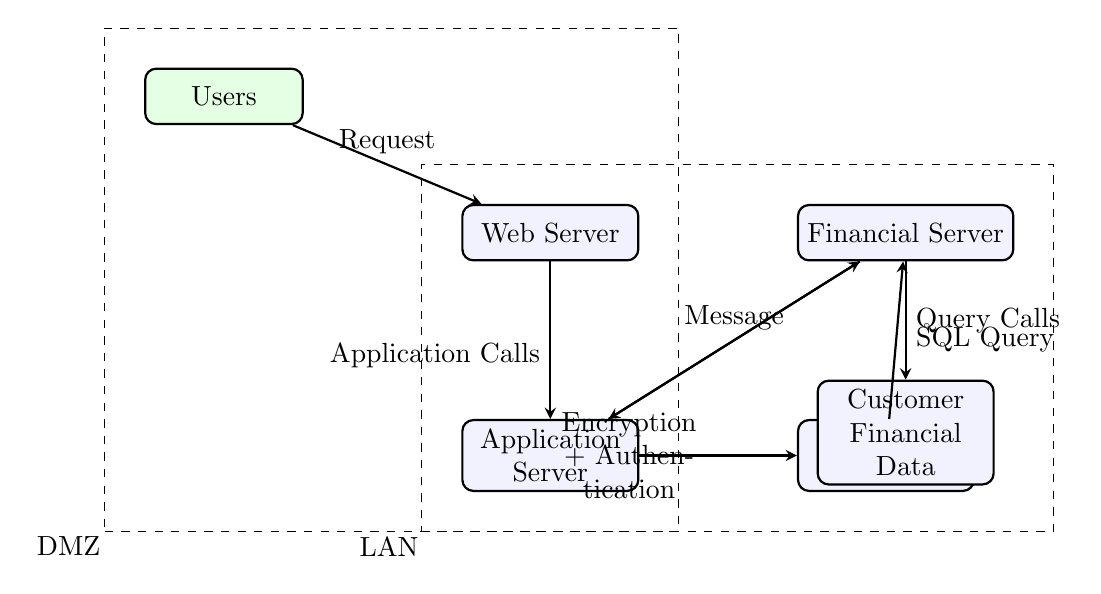
\begin{tikzpicture}[node distance=2.5cm and 3cm]
    
    % Nodes
    \node (user) [block, minimum width=2cm, fill=green!10] {Users};
    \node (web) [block, below right=1cm and 2cm of user, text width=2cm] {Web Server};
    \node (app) [block, below=2cm of web, text width=2cm] {Application Server};
    \node (db) [block, right=2cm of app, text width=2cm] {Database Server};
    \node (financial) [block, right=2cm of web, text width=2.5cm] {Financial Server};
    \node (customer) [block, below=1.5cm of financial, text width=2cm] {Customer Financial Data};

    % Boundaries
    \coordinate (DMZ_top) at (-1, 1);
    \coordinate (DMZ_bottom) at (4, -4.5);
    \node [draw, dashed, fit=(user) (web) (app), inner sep=0.5cm, label={[label distance=-0.1cm]south west:DMZ}] (DMZ) {};
    
    \coordinate (LAN_top) at (2, -0.5);
    \coordinate (LAN_bottom) at (9, -8.5);
    \node [draw, dashed, fit=(app) (db) (financial) (customer), inner sep=0.5cm, label={[label distance=-0.1cm]south west:LAN}] (LAN) {};

    % Arrows and Data Flow (Simplified Key Paths)
    \draw [arrow] (user) -- node[above] {Request} (web);
    \draw [arrow] (web) -- node[left, pos=0.6] {Application Calls} (app);
    \draw [arrow] (app) -- node[above] {Message} (financial);
    \draw [arrow] (financial) -- (app);
    
    \draw [arrow] (app) -- node[left, text width=2cm, align=center] {Encryption + Authentication} (db);
    \draw [arrow] (db) -- node[right, text width=2cm, align=center] {SQL Query} (financial);
    \draw [arrow] (financial) -- node[right] {Query Calls} (customer);

\end{tikzpicture}
\caption{Schematic Application Trust Boundaries and Data Flow}
\end{figure}

\subsubsection{Diagram 2: Banking Transaction Flow (Simplified DFD)}
This diagram illustrates a process flow, distinguishing between Authentication (AuthN) and Authorization (AuthZ), and showing how data interacts with policy checks.

\begin{figure}[H]
\centering
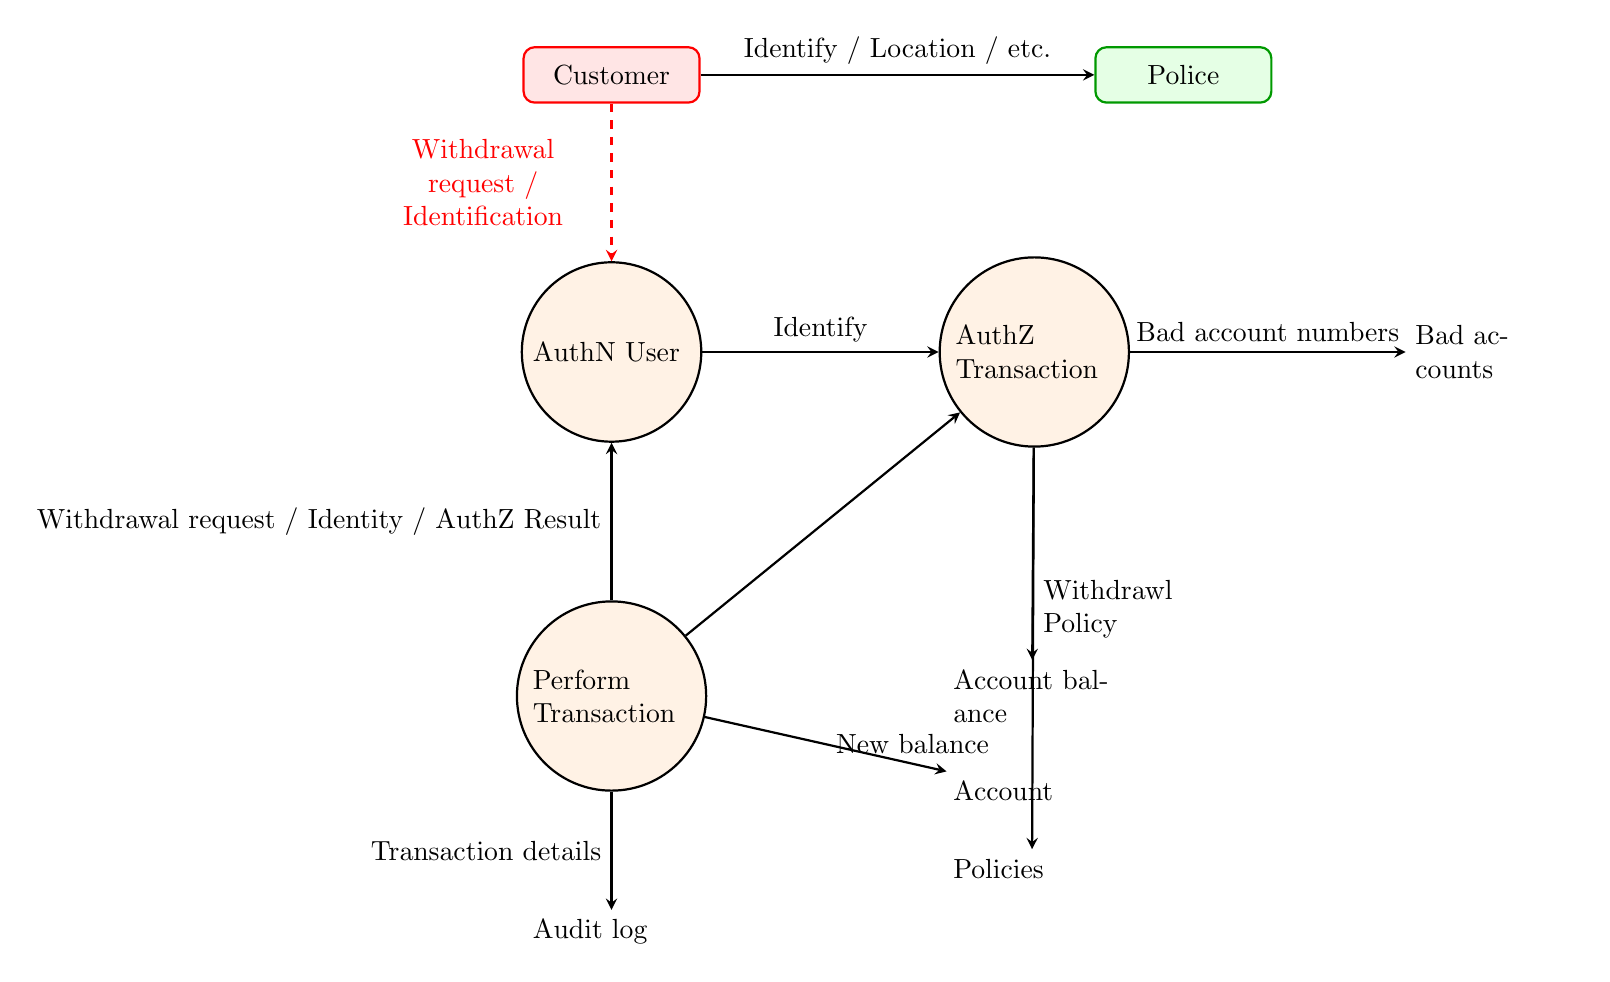
\begin{tikzpicture}[node distance=2cm and 4cm]

    % Entity
    \node (customer) [block, draw=red, fill=red!10, text width=2cm] {Customer};
    \node (police) [block, right=5cm of customer, draw=green!60!black, fill=green!10, text width=2cm] {Police};

    % Processes (Data Flow Diagram circles often represent processes, but here we use data style for the key security concepts)
    \node (authN) [data, below=2cm of customer, text width=2cm] {AuthN User};
    \node (authZ) [data, right=3cm of authN, text width=2cm] {AuthZ Transaction};
    \node (perform) [data, below=2cm of authN, text width=2cm] {Perform Transaction};

    % Data Stores/Outputs
    \node (audit) [below=1.5cm of perform, text width=2cm] {Audit log};
    
    \node (accountBalance) [right=3cm of perform, text width=2cm] {Account balance};
    \node (accountStore) [below=0.5cm of accountBalance, text width=2cm] {Account};
    \node (policies) [below=0.5cm of accountStore, text width=2cm] {Policies};
    \node (badAccounts) [right=3.5cm of authZ, text width=2cm] {Bad accounts};


    % Flows related to Customer/AuthN
    \draw [arrow, dashed, color=red] (customer) -- (authN) node[midway, left, text width=3cm, align=center] {Withdrawal request / Identification};
    \draw [arrow] (customer.east) -- (police) node[midway, above] {Identify / Location / etc.};

    % AuthN to AuthZ and back
    \draw [arrow] (authN) -- (authZ) node[midway, above] {Identify};
    \draw [arrow] (perform) -- (authN) node[midway, left] {Withdrawal request / Identity / AuthZ Result};

    % AuthZ checks
    \draw [arrow] (authZ.east) -- (badAccounts) node[midway, above] {Bad account numbers};
    \draw [arrow] (authZ) -- (accountBalance);
    \draw [arrow] (authZ) -- (policies) node[midway, above right, text width=2cm] {Withdrawl Policy};

    % Perform Transaction logic
    \draw [arrow] (perform) -- (accountStore) node[midway, right] {New balance};
    \draw [arrow] (perform) -- (audit) node[midway, left] {Transaction details};
    \draw [arrow] (perform) -- (authZ);

\end{tikzpicture}
\caption{Conceptual Threat Model: Banking Transaction Flow}
\end{figure}

\subsection{Security Assessment and Prevention}
The OWASP Software Assurance Maturity Model (SAMM) (\url{https://owaspsamm.org}) provides a framework for evaluating and improving the security practices of an organization.

To prevent insecure design, security must be integrated:
\begin{itemize}
    \item AppSec professionals must be involved in the design phase.
    \item Build a library of Secure Design patterns and reference code.
    \item Use Threat Modeling for critical systems to diagram authentication, access control, and authorization patterns.
    \item Document all Data Flows between systems.
    \item Create User Stories/Requirements to test against known attacks (SQL Injection, XSS, CSRF).
    \item Have PenTesters validate the design before deployment.
\end{itemize}

\section{A05: Security Misconfiguration (2021)}

Security Misconfiguration deals with systems and software that are improperly set up, leading to unnecessary exposure. This includes exploiting unpatched flaws, accessing unprotected files, and leveraging default configurations that grant excessive access.

\subsection{Prevention: Security Misconfiguration}
\begin{itemize}
    \item Work with administrators to ``Harden'' the server (``Lock it down'').
    \item Remove default accounts and credentials.
    \item Remove any unused services and turn off unnecessary ports.
    \item Add generalized error handling that hides system information (no stack traces).
    \item Take a least privilege approach to every component.
    \item Create a secure baseline (Gold Image) version of each OS.
    \item Utilize automated Security Testing and tools.
    \item Log Server and Application errors, and, critically, \textbf{review them regularly}.
\end{itemize}

\section{A06: Vulnerable and Outdated Components (2021)}

This risk category addresses vulnerabilities introduced by using outdated or flawed third-party components and libraries (3\textsuperscript{rd} party components). Since modern development relies heavily on these components, their security posture directly affects the application's overall security.

\subsection{Vulnerability Management Tools}
\begin{itemize}
    \item National Vulnerability Database (NVD): \url{https://nvd.nist.gov}
    \item OWASP Dependency Checker: \url{https://owasp.org/www-project-dependency-check/}
    \item Snyk.io: \url{https://snyk.io}
\end{itemize}

For Node.js projects, the Node Package Manager (NPM) offers:
\begin{verbatim}
npm ls [package name]
npm audit [fix]
npm update
\end{verbatim}

\subsection{Prevention: Vulnerable Components}
\begin{itemize}
    \item \textbf{Continuous Patching:} Integrate patching as a normal part of the development cycle (CI/CD pipelines).
    \item Use scanners in build/deployment pipelines to automatically check dependencies.
    \item Only use components from official sites/sources.
    \item Use a local, secured repository for development teams to pull vetted updates.
    \item Maintain scheduled releases for updates (e.g., quarterly).
    \item Do not allow frameworks to fall more than one or two major versions behind.
\end{itemize}

\section{A07: Identification and Authentication Failures (2021)}

This category covers weaknesses in managing user identities and confirming they are who they claim to be. Vulnerabilities often involve weak passwords, poor credential management, or insufficient session handling.

\subsection{Key Attack Vectors}
\begin{itemize}
    \item \textbf{Credential Stuffing:} Using large lists of previously leaked credentials (stolen from other sites, like those listed on \url{https://haveibeenpwned.com/}) to attempt logins.
    \item \textbf{Brute Force Attacks:} Trying large volumes of simple or commonly used passwords against accounts.
    \item \textbf{Weak Passwords:} Allowing default or easily guessable passwords (e.g., ``Password1'').
    \item \textbf{Weak Forgot-Password Processes:} Revealing user existence (enumeration) or emailing cleartext passwords.
\end{itemize}

\subsection{Password Security Protocols}
\begin{itemize}
    \item Plain text and encrypted passwords are fundamentally BAD because encrypted data can be decrypted.
    \item You must \textbf{ALWAYS} Hash passwords with a \textbf{RANDOM Salt} value unique for each user.
\end{itemize}

\subsection{Prevention: Broken Authentication}
\begin{itemize}
    \item Implement Complex Password Requirements (length $>$ 15 characters, special characters, mixed case).
    \item Implement Account Lockout after a small number of failed attempts.
    \item HASH passwords with a random SALT using a slow, modern algorithm (e.g., Argon2, bcrypt).
    \item Implement Multi-Factor Authentication (MFA) (e.g., Email, Text, QR code, RSA Token).
    \item Never email a user's password.
    \item Prevent user enumeration by giving a generic response to password reset requests (e.g., ``If an account exists, instructions were emailed'').
\end{itemize}

\section{A08: Software and Data Integrity Failures (2021)}

This category addresses the risks associated with code and infrastructure that fail to protect against integrity violations, particularly during updates and deployment.

\subsection{Prevention: Data Integrity Failures}
\begin{itemize}
    \item Use Digital Signatures to validate who created software updates.
    \item Manage internal package repositories for 3\textsuperscript{rd} party controls.
    \item \textbf{Integrity Check:} After deployment, calculate and compare HASHes (checksums) on files/folders to detect tampering.
    \item Manual Code Reviews of all critical changes.
    \item Harden CI/CD pipelines to restrict access and avoid storing credentials within them.
\end{itemize}

\section{A09: Security Monitoring and Logging Failures (2021)}

This item highlights that insufficient logging, monitoring, and active alerting prevents timely detection of security breaches. Logging must capture all traffic and activity, and logs must be secured away from the monitored system.

\subsection{Logging Best Practices}
\begin{itemize}
    \item Log normal traffic (successful paths) and all errors/exceptions.
    \item Use a centralized tool (like Splunk) to manage and review logs.
    \item \textbf{NEVER Log PII:} Avoid logging sensitive data like PII, Credit Cards, Tokens, or Passwords.
    \item \textbf{Monitoring is Essential:} Logging is \textbf{WORTHLESS} unless logs are reviewed daily for errors.
    \item Implement alerting systems for certain thresholds or abnormal traffic.
    \item Ensure high-value transactions have detailed, tamper-proof audit trails (e.g., append-only database tables).
\end{itemize}

\section{A10: Server-Side Request Forgery (SSRF) (2021)}

SSRF re-entered the Top 10 due to increased exploitation potential, particularly in cloud environments. SSRF occurs when a web application fetches a remote resource (or internal resource) without validating the user-supplied URL.

\subsection{Vulnerability and Prevention}
\begin{itemize}
    \item \textbf{Vulnerability:} SSRF allows attackers to force the server to connect to internal services or access sites the user shouldn't reach. The Panera Bread Hack (accessing user data by changing a sequential ID) is often a form of SSRF when an API endpoint processes the ID without validation.
    \item \textbf{Prevention:} Need to rigorously validate and sanitize user input that may contain URLs or resource identifiers. Implement strong allow-lists (whitelists) and deny-lists (blacklists) against internal IP ranges.
\end{itemize}

\end{document}
